\section{Spezifikation der Anwendung}
In diesem Kapitel werden die Anforderungen an das System und die daraus resultierenden Anwendungsfälle beschrieben.
Anschließend wird eine System-Abgrenzung vorgenommen, sowie auf die inhaltliche Gestaltung der Anwendung eingegangen.

\subsection{Anforderungen}
Die Kernanforderung an das System ist es, dem Benutzer zu ermöglichen, sich Artikel anzuschauen und diese bestellen zu können.
Darüberhinaus soll es einem Administrator möglich sein, neue Artikel anzulegen oder bestehende zu löschen.
Dafür ist die Implementierung eines Rollensystems nötig, um die Benutzergruppen unterscheiden zu können.

Für die Bestellung von Artikeln ist es nötig, dass sich ein Benutzer in der Anwendung registrieren und seine persönlichen Daten angeben kann.
Um eine Bestellung aufzugeben muss sich der registrierte Benutzer am System anmelden können.
Die detaillierte Beschreibung der dafür benötigten Anwendungsfälle findet sich in Kapitel \ref{usecases}.
\subsection{Nichtfunktionale Anforderungen}
Die Anwendung sollte von allen gängigen Browsern in neueren Versionen sowie auf mobilen Geräten darstellbar sein.
Sensible Daten, wie die persönlichen Daten der Anwender, müssen vor unbefugtem Zugriff geschützt sein.

Im Fehlerfall soll der Benutzer über Hinweise darauf aufmerksam gemacht werden.
Dabei sollen interne Fehlermeldungen des Servers, sowie unverständliche Fehlercodes sollen vor dem Anwender verborgen werden.
Um die Benutzerfreundlichkeit der Anwendung zu sichern, sollte sich die Antwortzeit des Servers in einem vertretbaren Rahmen bewegen (Richtwert 3 Sekunden).
\subsection{Hauptanwendungsfälle}\label{usecases}
Das folgende Diagramm zeigt die Anwendungsfälle für den Benutzer und Administrator, sowie die jeweils beteiligten System-Komponenten.
Die Anwendungsfälle werden im Anschluss im Einzelnen betrachtet.
\begin{figure}[ht!]
	\centering
	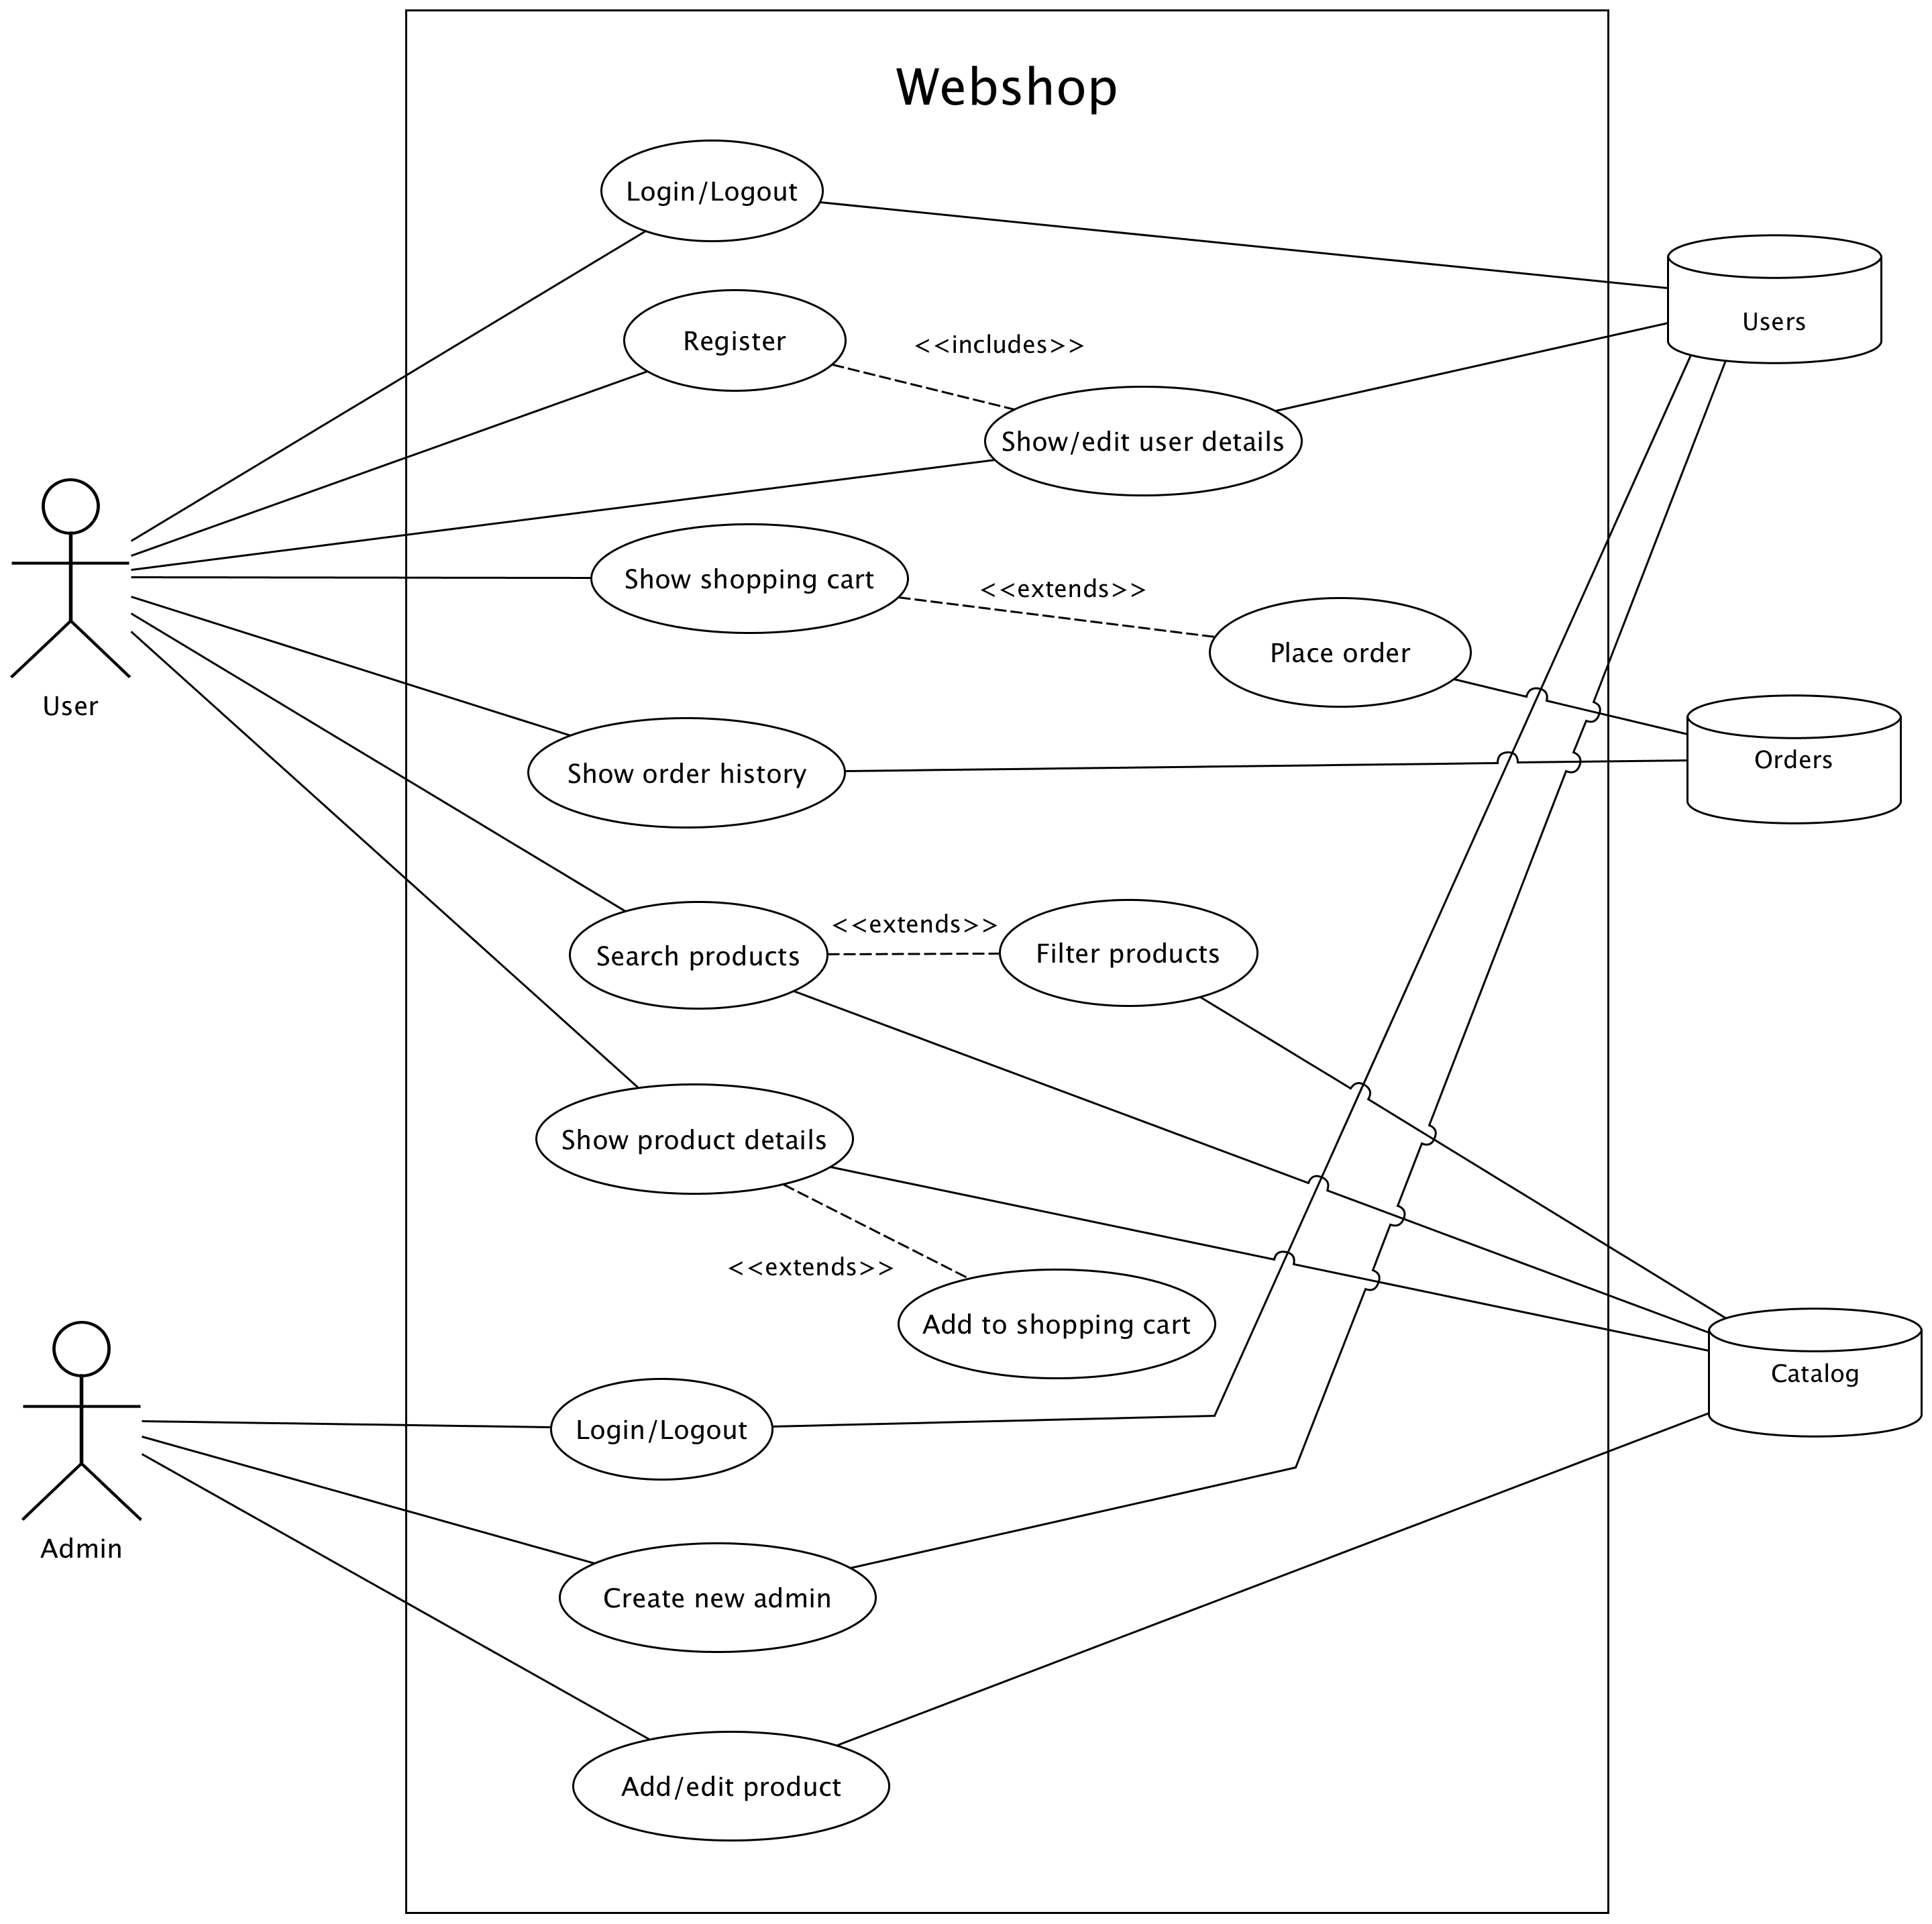
\includegraphics[width=\linewidth]{bilder/kap4/use_cases}
	\caption{Anwendungsfalldiagramm mit den Hauptanwendungsfällen}
	\label{fig:usecases}
\end{figure}

\subsubsection{Benutzer- bzw. Kunden-Anwendungsfälle}
\paragraph{Register (Registrierung)}
Ein Benutzer soll sich durch Angabe seiner persönlichen Daten beim System registrieren können.
Die dafür nötigen Pflichtangaben sind:
\begin{itemize}
\item Anrede
\item Vorname
\item Nachname
\item Geburtsdatum
\item E-Mail-Adresse
\item Passwort
\item Straße und Hausnummer
\item Stadt
\item Postleitzahl
\item Land
\end{itemize}
Zusätzlich soll es bei der Registrierung möglich sein, eine abweichende Lieferadresse einzugeben.
Nach der Registrierung muss es dem Benutzer möglich sein, sich am System anzumelden.
Um Artikel anschauen zu können und sie in den Warenkorb zu legen, muss ein Besucher der Seite nicht registriert oder angemeldet sein.

\paragraph{Login/Logout}
Registrierte Nutzer können sich durch die Eingabe ihrer E-Mail-Adresse und ihrem Passwort im Shop einloggen.
Bei einer fehlerhaften Eingabe soll eine Meldung ausgegeben werden.
Der Login ist Voraussetzung für folgende weitere Use Cases: Anzeigen/Bearbeiten der persönlichen Informationen, Bestellung aufgeben und Bestellhistorie einsehen.
Außerdem muss beim Einloggen auch der Warenkorb des jeweiligen Benutzers geladen werden, da dieser Artikel enthalten kann, die der User beim letzten Besuch des Shops hineingelegt hat.
Beim Logout wird der Benutzer wieder abgemledet und kann ohne einen erneuten Login nicht mehr auf seine Daten zugreifen oder die benutzerspezifischen Anwendungsfälle ausführen.

\paragraph{Show/edit user details (Anzeigen/Bearbeiten der persönlichen Informationen)}
Einem eingeloggten Benutzer soll es möglich sein, seine persönlichen Daten einzusehen und zu ändern.
Eine übersichtliche Seite mit allen Informationen und Funktionalitäten soll ihm dafür zur Verfügung stehen.

\paragraph{Show shopping cart (Warenkorb anzeigen)}
\paragraph{Add to shopping cart (Zum Warenkorb hinzufügen)}
\paragraph{Place order (Bstellung aufgeben)}
\paragraph{Show order history (Bestellhistorie einsehen)}
\paragraph{Search products (Artikelsuche)}
\paragraph{Filter products (Artikel filtern)}
\paragraph{Show product details (Detailansicht eines Artikels)}

\subsubsection{Administrator-Anwendungsfälle}
\subsection{System-Abgrenzung}
Diagramm, Grenzen stecken
\subsection{Inhaltliche Definition}
Wolle